% MIT License

% Copyright (c) 2019-2020 Simon Crase

% Permission is hereby granted, free of charge, to any person obtaining a copy
% of this software and associated documentation files (the "Software"), to deal
% in the Software without restriction, including without limitation the rights
% to use, copy, modify, merge, publish, distribute, sublicense, and/or sell
% copies of the Software, and to permit persons to whom the Software is
% furnished to do so, subject to the following conditions:

% The above copyright notice and this permission notice shall be included in all
% copies or substantial portions of the Software.

% THE SOFTWARE IS PROVIDED "AS IS", WITHOUT WARRANTY OF ANY KIND, EXPRESS OR
% IMPLIED, INCLUDING BUT NOT LIMITED TO THE WARRANTIES OF MERCHANTABILITY,
% FITNESS FOR A PARTICULAR PURPOSE AND NONINFRINGEMENT. IN NO EVENT SHALL THE
% AUTHORS OR COPYRIGHT HOLDERS BE LIABLE FOR ANY CLAIM, DAMAGES OR OTHER
% LIABILITY, WHETHER IN AN ACTION OF CONTRACT, TORT OR OTHERWISE, ARISING FROM,
% OUT OF OR IN CONNECTION WITH THE SOFTWARE OR THE USE OR OTHER DEALINGS IN THE
% SOFTWARE.

\documentclass[]{article}
\usepackage{caption,subcaption,graphicx,float,url,amsmath,amssymb,tocloft,cancel,amsthm}
\usepackage[hidelinks]{hyperref}
\usepackage[toc,acronym,nonumberlist]{glossaries}
\usepackage{titling}
\setacronymstyle{long-short}
\usepackage{glossaries-extra}
\graphicspath{{figs/}} 
\setlength{\cftsubsecindent}{0em}
\setlength{\cftsecnumwidth}{3em}
\setlength{\cftsubsecnumwidth}{3em}
% I snarfed the next line from Stack exchange
% https://tex.stackexchange.com/questions
%    /42726/align-but-show-one-equation-number-at-the-end
% It allows me to suppress equation numbers with align*,
% then selectively add equation numbers
% for lines that I want to reference slsewhere
\newcommand\numberthis{\addtocounter{equation}{1}\tag{\theequation}}
\newtheorem{thm}{Theorem}
% Add logo at start of document


%opening
\title{
	Notes from \\
	Computation in Complex Systems
}
\author{Simon Crase (compiler)\\simon@greenweaves.nz}

\makeglossaries


%\loadglsentries{glossary-entries}

\renewcommand{\glstextformat}[1]{\textbf{\em #1}}

\begin{document}

\maketitle

\begin{abstract}
   These are my notes from Computation in Complex Systems\
   The content and images contained herein are the intellectual property of the Santa Fe Institute, with the exception of any errors in transcription, which are my own.
   These notes are distributed in the hope that they will be useful,
   but without any warranty, and without even the implied warranty of
   merchantability or fitness for a particular purpose. All feedback is welcome,
   but I don't necessarily undertake to do anything with it.\\
   \LaTeX source for this week's lectures can be found at\\
   \url{https://github.com/weka511/complexity/tree/master/origins}.
\end{abstract}

\setcounter{tocdepth}{2}
\tableofcontents

\listoffigures

\newglossaryentry{gls:3:SAT}{
	name={$3-SAT$},
	description={Given a set of \glspl{gls:clause} with 3 variables (or negated variables) each, e.g. $(x_1 \lor \bar{x_2} \lor x_3) \land (x_2 \lor x_{17} \lor \bar{x_{23}}) \land...$ is there a set $\{x_i\}$ such that all clauses are satisfied?}}

\newglossaryentry{gls:clause}{
	name={clause},
	description={In logic, a clause is an expression formed from a finite collection of literals (atoms or their negations) }}

\newglossaryentry{gls:eulerian:path}{
	name={Eulerian path},
	description={In graph theory, an Eulerian path is a path in a finite graph that visits every edge exactly once (allowing for revisiting vertices) }}

\newglossaryentry{gls:eulerian:cycle}{
	name={Eulerian cycle},
	description={Similarly, an Eulerian circuit or Eulerian cycle is an \gls{gls:eulerian:path} that starts and ends on the same vertex. }}

\newglossaryentry{gls:Hamiltonian:cycle}{
	name={Hamiltonian cycle},
	description={If a \gls{gls:Hamiltonian:path} exists whose endpoints are adjacent, then the resulting graph cycle is called a Hamiltonian cycle (or Hamiltonian cycle) }}

\newglossaryentry{gls:Hamiltonian:path}{
	name={Hamiltonian path},
	description={A Hamiltonian path, also called a Hamilton path, is a graph path between two vertices of a graph that visits each vertex exactly once }}

\newglossaryentry{gls:NonDP}{
	name={Non-deterministic Polynomial Time},
	description={we can \emph{check} a solution efficiently}}

\newglossaryentry{gls:NP:complete}{
	name={NP-Complete},
	description={It turns out that there are problems $B$ in \gls{gls:NP} such that any other problem $A$  in \gls{gls:NP} can be \gls{gls:reduced} to $B$: $A \le B \forall A \in NP$. Such a $B$ is said to be NP-Complete}}

\newglossaryentry{gls:O}{
	name={O},
	description={$f(n)=O(n^3)$ means: when $n$ is large $f(n)$ scales as $n^3$ or less. Formally:
	\begin{align*}
		f(n) =& O(g(n))\\
		\equiv&	\;\; \exists C, n_0 \text{ such that}\\
		 \forall n>n_0, f(n) \le& Cg(n)
	\end{align*}}}

\newglossaryentry{gls:o}{
	name={o},
	description={$f$ grows more slowly than $g$: $f/g \rightarrow 0 \text{ as } n\rightarrow \infty$}}

\newglossaryentry{gls:Omega}{
	name={$\Omega$},
	description={$f$ grows at least as fast as $g$: $g=O(f)$ : $f/g \cancel{\rightarrow} 0 \text{ as } n\rightarrow \infty$}}

\newglossaryentry{gls:Polynomial}{
	name={Polynomial Time},
	description={we can find a solution efficiently}}

\newglossaryentry{gls:reduced}{
	name={reduced},
	description={$A$ can be \emph{reduced} to $B$, or $A \le B$, if there is a polynomial algorithm that translated instances of $A$ to instances of $B$, so the yes/no answer stays the same. }}

\newglossaryentry{gls:Theta}{
	name={$\Theta$},
	description={$f$ and $g$ grow the same way: $g=O(f)$ and $f=O(g)$ or $f/g \rightarrow C>0\text{ as } n\rightarrow \infty$}}


\newacronym[see={[Glossary:]{gls:Polynomial}}]{gls:P}{P}{Polynomial\glsadd{gls:Polynomial}}

\newacronym[see={[Glossary:]{gls:NonDP}}]{gls:NP}{NP}{Non-deterministic Polynomial\glsadd{gls:NonDP}}

\section{Easy \& Hard}

\cite[Chapters 1,2,4]{moore2011nature}

For theorists, polynomial vs. exponential is the mark of insight: we have found some structure in the problem that we can use.

\subsection{Two Kinds of Paths}

\begin{figure}[H]
	\caption{Eulerian paths}
	\begin{subfigure}[t]{0.54\textwidth}
		\caption{The 7 bridges of K\"onigsberg: can we cross each bridge only once? One strategy is brute force search.}
		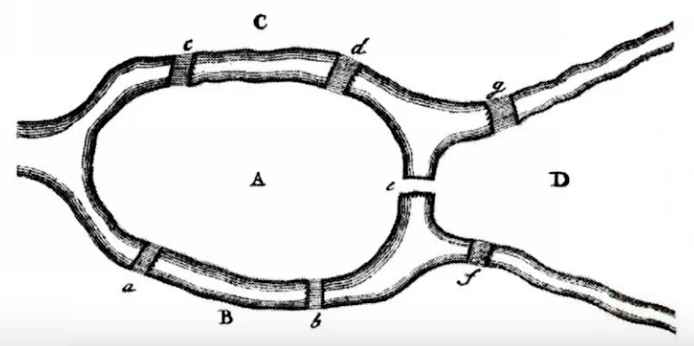
\includegraphics[width=\textwidth]{euler}
	\end{subfigure}
	\begin{subfigure}[t]{0.54\textwidth}
		\caption{Euler: if a tour exists, at most 2 noded can have an odd number of bridges, so no tour is possible. Much faster.}
		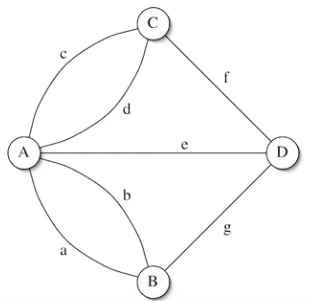
\includegraphics[width=\textwidth]{euler2}
	\end{subfigure}
\end{figure}

\begin{figure}[H]
	\begin{center}
		\caption{Hamiltonian Path: visit each node once}
		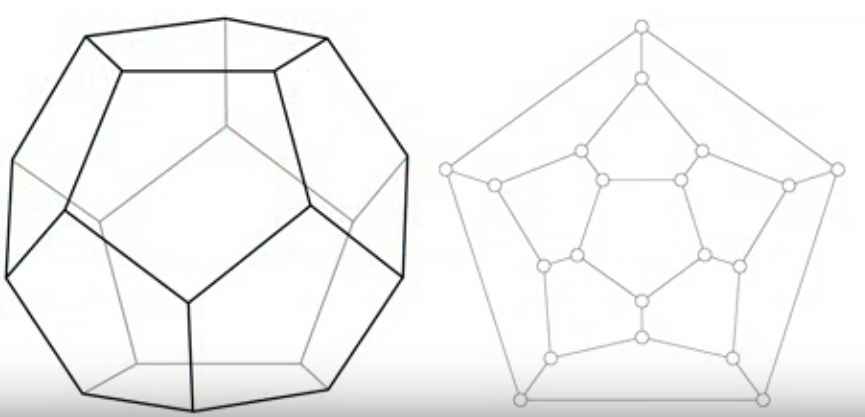
\includegraphics[width=\textwidth]{Hamiltonian}
	\end{center}
\end{figure}

\subsection{Polynomials vs. Exponentials}

\subsection{Divide and Conquer}

\subsection{Big O and All that}

\subsection{When the details don't matter}

\section{Algorithms and Landscapes}
\cite[Chapter 2]{moore2011nature}

\subsection{Divide and Conquer Redux}

\subsection{Dynamic Programming}

\begin{align*}
	d(s,t)=& \min(d(s^\prime,t)+1, d(s,t^\prime)+1,d(s^\prime,t^\prime) + \delta(s_1,t_1)) \text{ , where}\\
	d(s,t)=& \text{ number of changes to convert $s$ to $d$}\\
	s^\prime=& \text{ string $s$ with 1st character, $s_1$ removed}\\
	t^\prime=& \text{ string $t$ with 1st character, $t_1$ removed}
\end{align*}

There are only $n^2$ sub-problems: polynomial time.

\subsection{Greedy Algorithms}

\begin{figure}[H]
	\caption{Minimum Spanning Tree}
	\begin{subfigure}[t]{0.45\textwidth}
		\caption{e.g. power lines}
		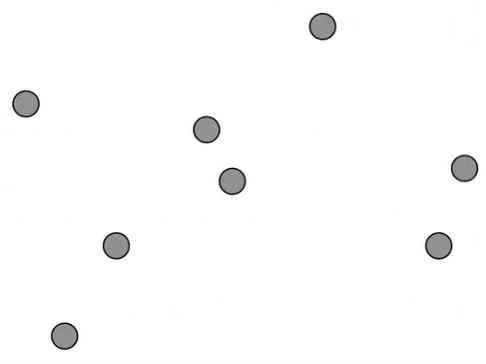
\includegraphics[width=\textwidth]{mst1}
	\end{subfigure}
	\;\;\;
	\begin{subfigure}[t]{0.45\textwidth}
		\caption{Start by adding the shortest edge}
		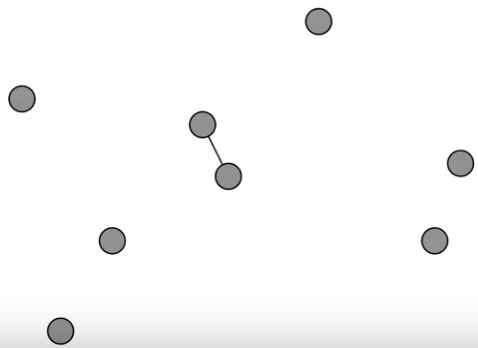
\includegraphics[width=\textwidth]{mst2}
	\end{subfigure}
	\begin{subfigure}[b]{0.45\textwidth}
		\caption{At each step, add the shortest edge that doesn't complete a cycle}
		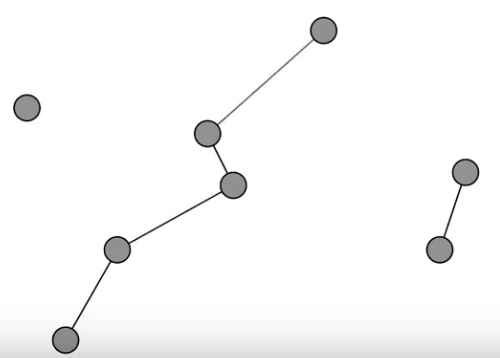
\includegraphics[width=\textwidth]{mst3}
	\end{subfigure}
	\;\;\;
	\begin{subfigure}[b]{0.45\textwidth}
		\caption{The complete tree}\label{fig:mst4}
		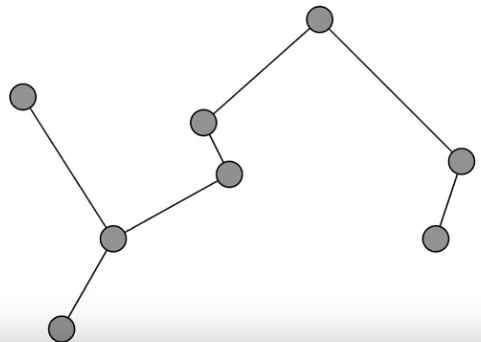
\includegraphics[width=\textwidth]{mst4}
	\end{subfigure}
\end{figure}

Clearly Figure \ref{fig:mst4} is \emph{a} spanning tree, but how do we know it is minimal?

\begin{figure}[H]
	\caption{How do we know Figure \ref{fig:mst4} is minimal?}
	\begin{subfigure}[b]{0.30\textwidth}
		\caption{Let $e$ be the shortest edge that doesn't complete a cycle, and suppose that the minimum spanning tree $T$ doesn't contain $e$}
		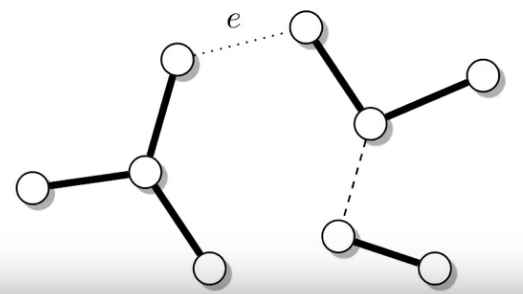
\includegraphics[width=\textwidth]{mst5}
	\end{subfigure}
	\;\;\;
	\begin{subfigure}[b]{0.30\textwidth}
		\caption{Then there must be some other path from one end of $e$ to another that goes through a longer edge $e^\prime$.}
		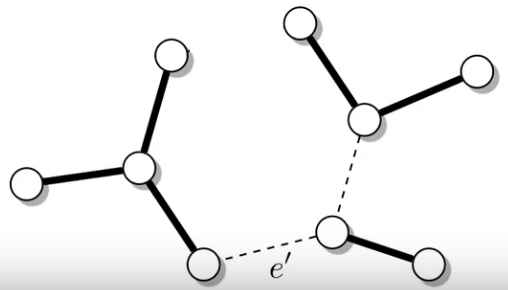
\includegraphics[width=\textwidth]{mst6}
	\end{subfigure}
	\;\;\;
	\begin{subfigure}[b]{0.30\textwidth}
		\caption{But then we could reduce the total length by deleting $e^\prime$ and adding $e$--a contradiction.}
		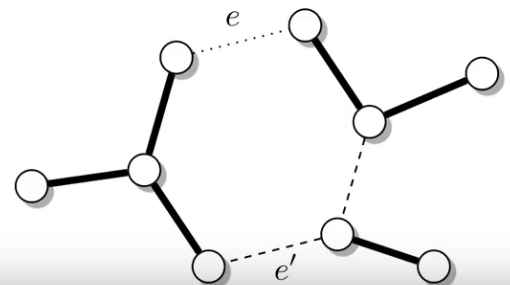
\includegraphics[width=\textwidth]{mst7}
	\end{subfigure}
\end{figure}

Greed isn't always good, or even very often good--Figures \ref{fig:greedy:tsp} and \ref{fig:lessgreedy:tsp}.
\begin{figure}[H]
	\caption{Travelling Salesman Problem}
	\begin{subfigure}[t]{0.45\textwidth}
		\caption{Greedy solution to Travelling Salesman Problem}\label{fig:greedy:tsp}
		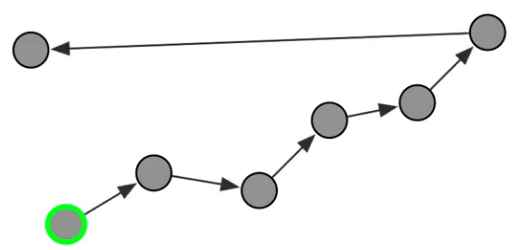
\includegraphics[width=\textwidth]{tsp1}
	\end{subfigure}
	\;\;\;
	\begin{subfigure}[t]{0.45\textwidth}
		\caption{A less Greedy solution is somewhat better}\label{fig:lessgreedy:tsp}
		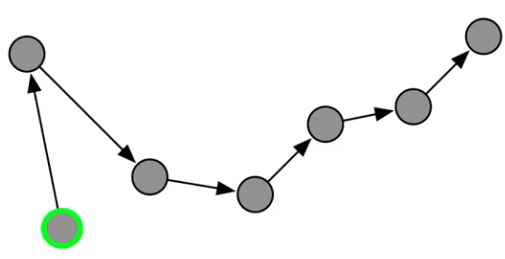
\includegraphics[width=\textwidth]{tsp2}
	\end{subfigure}
\end{figure}

\subsection{Landscapes}

\subsubsection{Greedy Algorithms and the Fitness Landscape}

\begin{figure}[H]
	\caption{Greedy Algorithms and the Fitness Landscape}
	\begin{subfigure}[t]{0.4\textwidth}
		\caption{A greedy algorithm works well if the Fitness Landscape looks like Fuji-San}
		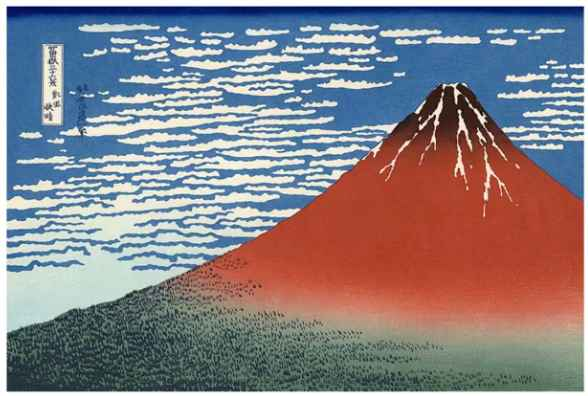
\includegraphics[width=\textwidth]{fujisan}
	\end{subfigure}
	\;\;\;
	\begin{subfigure}[t]{0.55\textwidth}
		\caption{A Greedy solution doesn't work well if there are many local optima where we can get stuck: it cannot cross a valley to get to a higher peak.}
		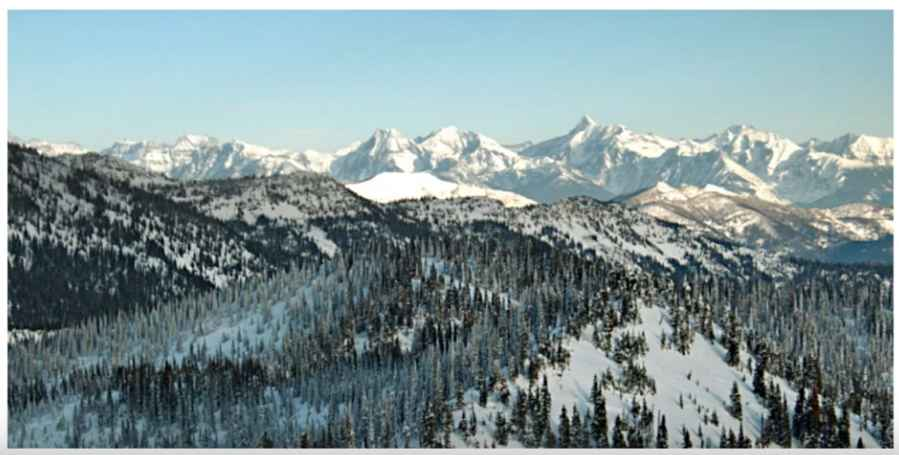
\includegraphics[width=\textwidth]{rockies}
	\end{subfigure}
\end{figure}

\subsubsection{Reorganizing the Landscape}

What defines the neighbourhood? When is one solution close to another?

\begin{figure}[H]
	\caption[Maxflow: determine the maximum flow from $s$ to $t$]{Maxflow: take a network such as \ref{fig:maxflow1} and determine the maximum flow from $s$ to $t$. We can see that we can eliminate local optima by allowing a new kind of move. By expanding our idea of what kins of solutions are neighbours we reorganize the landscape!}
	\begin{subfigure}[t]{0.4\textwidth}
		\caption{Each edge has a capacity}\label{fig:maxflow1}
		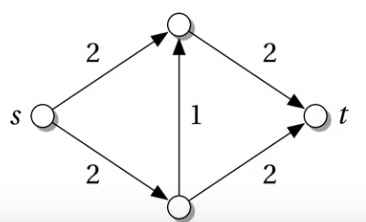
\includegraphics[width=\textwidth]{maxflow1}
	\end{subfigure}
	\;\;\;
	\begin{subfigure}[t]{0.55\textwidth}
		\caption{Greedy: push more flow along a channel with excess capacity. But we can get stuck at a local optimum. Here we have three units flowing--we are at a local optimum.}\label{fig:maxflow2}
		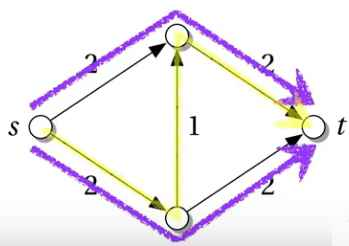
\includegraphics[width=\textwidth]{maxflow2}
	\end{subfigure}
	\;\;\;
	\begin{subfigure}[t]{0.45\textwidth}
		\caption{We should have done this instead}\label{fig:maxflow3}
		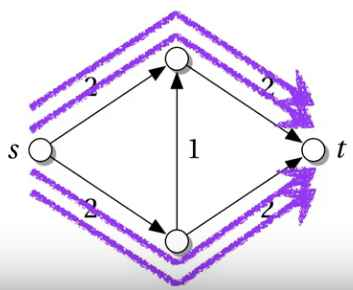
\includegraphics[width=\textwidth]{maxflow3}
	\end{subfigure}
	\;\;\;
	\begin{subfigure}[t]{0.45\textwidth}
		\caption{Allow reverse edges to cancel previous flow: now if we add to Figure \ref{fig:maxflow2} we get the optimum--Figure \ref{fig:maxflow3}. If we allow this type of move we can never get stuck: there are no local optima.}
		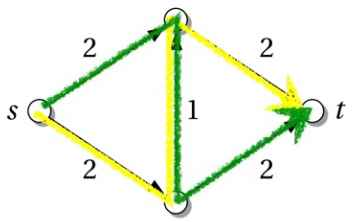
\includegraphics[width=\textwidth]{maxflow4}
	\end{subfigure}
\end{figure}

This won't always work. Some problems are inherently bumpy.

\subsection{Reductions and Translations}

\begin{figure}[H]
	\caption[Reducing one problem into another]{Reducing one problem into another. We want a perfect bipartite matching, where everyone has a partner. This is a subset of the edges of this graph, so everyone on one side is connected to exactly one person on the other. There are $n!$ possible matchings.}
	\begin{subfigure}[t]{0.3\textwidth}
		\caption{Bipartite Graph. }
		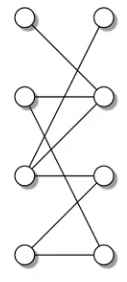
\includegraphics[width=\textwidth]{bpg1}
	\end{subfigure}
	\;\;\;
	\begin{subfigure}[t]{0.65\textwidth}
		\caption{We can transform the problem to max flow. Each compatible couple becomes an edge with flow 1.}
		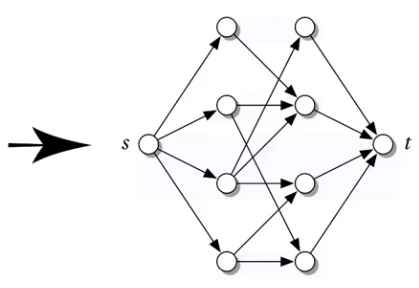
\includegraphics[width=\textwidth]{bpg2}
	\end{subfigure}
\end{figure}

\begin{thm}
	If all the flows have integral capacities, the solution is also integral.
\end{thm}

In terms of complexity, Bipartite Matching $\le$ Max Flow.


\begin{figure}[H]
	\caption{Shortest Path}
	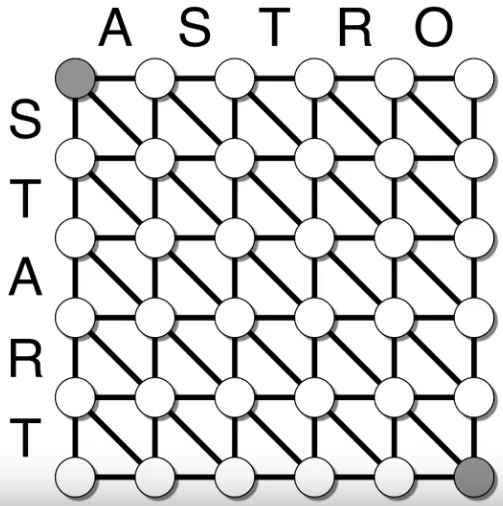
\includegraphics[width=0.8\textwidth]{sp1}
\end{figure}

\subsection{Lessons So Far}

\subsection{The Best of All Possible Algorithms}

\subsection{Complexity Wrap-Up}

\begin{itemize}
	\item \emph{Systems} aren't simple or complex; questions about them are.
	\item Intrinsic complexity of a problem: the running time, or memory, or other resource, of the \emph{best possible algorithm}; an objective mathematical fact.
	\item Upper bounds are easy: just give an algorithm.
	\item Lower bounds are hard.
	\item Lower bounds show that one problem is at least as easy (or hard) as another. 
\end{itemize}

\section{P versus NP}
\cite[Chapters 4-6]{moore2011nature}, \cite{sep-computability}

\subsection{Finding versus Checking}

Some problems can be solved in polynomial time, while other require a brute-force search, which is typically exponential. In the P vs. NP question we deal with ''needles in haystacks'': finding a solution, or telling whether there is one seems hard, by checking a solution is easy.

\begin{figure}[H]
	\begin{center}
		\caption[Hamiltonian path]{\gls{gls:Hamiltonian:path}. We don't know how to solve it in polynomial time, but we can easily check a proposed solution.}\label{fig:PNP1}
		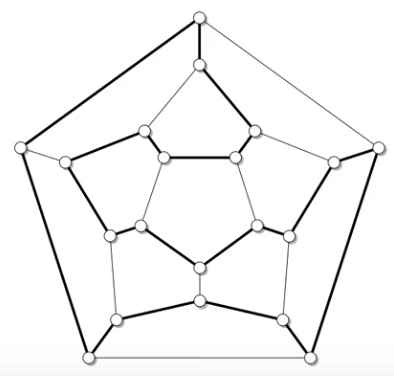
\includegraphics[width=0.8\textwidth]{PNP1}
	\end{center}
\end{figure} 

\begin{itemize}
	\item \gls{gls:P}: \glsdesc{gls:Polynomial}
	\item \gls{gls:NP}: \glsdesc{gls:NonDP}
\end{itemize}

\begin{figure}[H]
	\begin{center}
		\caption[Complexity Classes]{Complexity Classes. We \emph{know} that $P \subseteq NP$, and we \emph{believe} that $P \subset NP$}\label{fig:PNP2}
		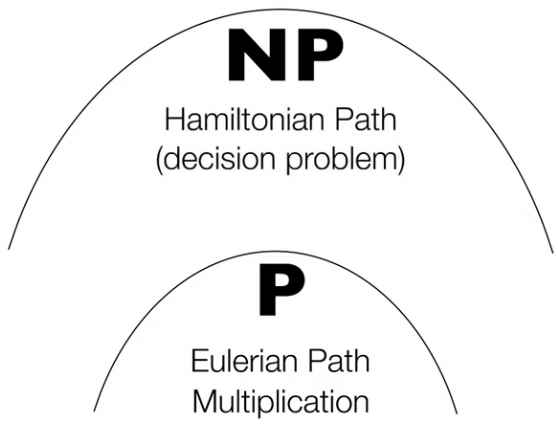
\includegraphics[width=0.8\textwidth]{PNP2}
	\end{center}
\end{figure}

We'll focus on classes of decision problems: not \emph{does this graphs have a \gls{gls:Hamiltonian:path}}, but \emph{can we find a \gls{gls:Hamiltonian:path} for \emph{\gls{gls:Hamiltonian:path}} graph}. We consider \gls{gls:NP:complete} problems.

We say that \glsdesc{gls:reduced} \glsdesc{gls:NP:complete}

But if $A \le B$ and $A$ is hard, them $B$ must be hard too: so $B$ is one of the hardest problems in \gls{gls:NP}. We can therefore focus on one  \gls{gls:NP}: if $B\in NP$ we would know that $P=NP$. Conversely, if $P \ne NP$, $B$ cannot be solved in polynomial time.

Now the Hamiltonian Path problem is NP-Complete: how can such a simple problem represent all \gls{gls:NP} problems?

\subsection{Circuits and Formulae}

Figure \ref{fig:satisfying} illustrates how the question ''is there a \gls{gls:Hamiltonian:path}'' can be transformed to ''are there values for the inputs that make to output \textbf{true}?''
\begin{figure}[H]
	\begin{center}
		\caption{Satisfying a circuit}
		\begin{subfigure}[b]{0.45\textwidth}
			\caption{Satisfying a circuit: any program that tests solutions--e.g. to \gls{gls:Hamiltonian:path}--can be compiled into a Boolean circuit--bits!}\label{fig:satisfying}
			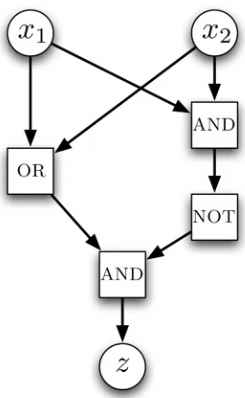
\includegraphics[width=\textwidth]{satisfy}
		\end{subfigure}
		\begin{subfigure}[b]{0.45\textwidth}
			\caption{Add variables representing the truth values of the wires.}\label{fig:add:variables}
			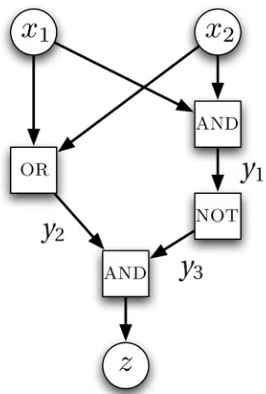
\includegraphics[width=\textwidth]{add-variables}
		\end{subfigure}
	\end{center}
\end{figure}

\begin{align*}
	y = x_1 \land& x_2 \equiv (x_1\lor \bar{y_1}) \land (x_1\lor \bar{y_2}) \land (\bar{x_1} \lor \bar{x_2} \lor y_1)
\end{align*}

We have converted the problem of checking a problem to a program, and than into a problem of checking Boolean expressions. We have therefore reduced out original problem to an instance of \gls{gls:3:SAT}, one of the original 6 \gls{gls:NP:complete} problems.
\glsdesc{gls:3:SAT} k-SAT is ($k$ variables per clause) is \gls{gls:NP:complete} $\forall k \ge 3$.

If \gls{gls:3:SAT} were easy:
\begin{itemize}
	\item we could take any \gls{gls:NP} problem;
	\item write a program that checks a solution;
	\item convert to a circuit;
	\item convert to a 3-SAT formula;
	\item use our efficient 3-SAT solver to solve the original problem;
	\item so if $3-SAT \in P$ then $P=NP$.
	\item If $P\ne NP$, 3-SAT cannot be solved in polynomial time.
\end{itemize}

\begin{thm}
	k-SAT $\le$ 3-SAT
\end{thm}

\begin{proof}
	We can break k-clauses down into 3-clauses, by adding new variables $\{z_i\}$, e.g.:
	\begin{align*}
		(x_1 \lor x_2 \lor x_3 \lor x_4 \lor x_5) =& (x_1 \lor x_2 \lor z_1) \land (\bar{z_1} \lor x_3 \lor z_2) \land (\bar{z_2} \lor x_4 \lor x_5)
	\end{align*}
	so we get 3-SAT clauses. They are good logical building blocks: this isn't true for 2-SAT clauses. A 3-SAT clause has ''chemistry'' and triggers a search. 2-SAT $\in$ P.
\end{proof}
\subsection{More NP-complete Problems}

\subsection{P versus NP Problem}

\subsection{Existence and Nonexistence }

\subsection{Above and Beyond}

\section{Worst-case, Natural, and Random}
\cite[Chapters 5,10]{moore2011nature}
\section{Computation Everywhere}
\cite[Chapter 7]{moore2011nature}
% end of text 

% glossary
\glsaddall
\printglossaries

% bibliography go here
 
\bibliographystyle{unsrt}
\addcontentsline{toc}{section}{Bibliography}
\bibliography{computations}

\end{document}
